\documentclass{article}
\usepackage{parskip}
\usepackage{amsmath}
\usepackage[dvipdfmx]{graphicx}
\usepackage{cleveref}

\newcommand{\myparagraph}[1]{\paragraph{#1}\mbox{}\\}

\begin{document}

ある長方形を3つの長方形に分割する方法は,
ある1辺に平行な2本の線分によって分割する方法(\cref{type-i})か,
各辺にそれぞれ平行な1本ずつの線分によって分割する方法(\cref{type-t})のいずれかのみである。
これらをそれぞれI型,T型と呼ぶことにする。

\begin{figure}[h]
    \begin{center}
        \begin{tabular}{c}
            \begin{minipage}{0.33\hsize}
                \begin{center}
                    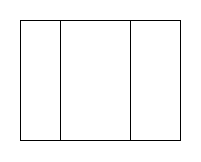
\includegraphics[width=100pt]{type-i.png}
                    \caption{I型}
                    \label{type-i}
                \end{center}
            \end{minipage}

            \begin{minipage}{0.33\hsize}
                \begin{center}
                    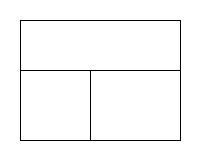
\includegraphics[width=100pt]{type-t.png}
                    \caption{T型}
                    \label{type-t}
                \end{center}
            \end{minipage}
        \end{tabular}
    \end{center}
\end{figure}

$\Delta S = S_{max} - S_{min}$とおく。
$H, W$の少なくとも一方が3で割り切れるならば,
I型の分割によってちょうど3等分することができ,
このように分割すれば$\Delta S = 0$である。
以下,$H, W$のいずれも3で割り切れないときを考える。

\myparagraph{[1] I型に分割するとき}

まず,縦の辺に平行な2本の線分を引いて分割する場合を考える。
$W = 2$のときはI型の分割が存在しないから,
2以上の整数$k$を用いて$W = 3k + 1$または$W = 3k - 1$と表せるときを考えればよい。

このとき,$\Delta S$が最小となるような
3つの長方形の横の長さの組は$k, k, k + 1$または$k, k, k - 1$であり,
このように分割すれば$\Delta S = H$ である。

横の辺に平行な2本の線分を引いて分割する場合も同様に考えて
$\Delta S = W$を得る。

したがって,I型の分割をするときの$\Delta S$の最小値は
\begin{equation*}
    \Delta S = \min \{H, W\}
\end{equation*}
である。

\myparagraph{[2] T型に分割するとき}

\end{document}
